\documentclass{article}

\usepackage{amsmath}
\usepackage{listings}
\usepackage{physics}
\usepackage{graphicx}
\usepackage{pdfpages}
\usepackage{svg}
\usepackage{hyperref}

\author{}
\date{}
\title{\vspace{-4cm}Introduction to GitHub}
\begin{document}
\maketitle
\section{Introduction to Git}
Git is an open source software for version control developed by the same guy that developed Linux, Linus Torvald. Git was developed to give software developers a protocol and system for version control that is fast and allows for collaborative work. GitHub is the most popular service built on the Git, its main value offering is that it hosts servers and streamlines the process of sharing and collaborating using the Git protocol, as well as having a GUI and desktop program that allows you to use Git without using command line. Git services can be also used separate of GitHub, either in competing services like GitLab, or in a self run Git server you can set up your self.
\section{Git Features}
\subsection{Version Control}
Version control allows you to create save states (called commits) that keep track of the changes made to your code base over time, should be named according to the updates made to the code base,and gives you the ability to return to any of these saved states for any reason (like breaking your code so it doesn't compile/run). Version control is not only useful as a personal tool, to act as changelog or to return to save states, but is also very useful when teaching the code base to a new user/developer. New users can see when certain features were added to the code, how they were added, and how the code developed.
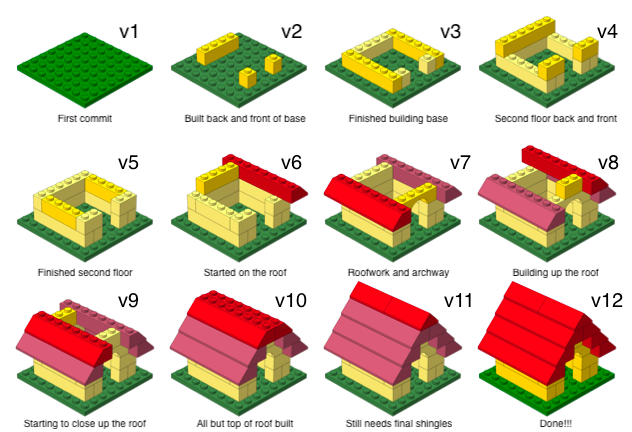
\includegraphics[width=\textwidth]{lego-steps-commit-messages.png}

\subsection{Branches}
While version control acts as saved states, branches are different universes where you can test changes or updates to the code base before either merging them together, or continuing a new project with different features on a new branch. After making a pull request, the current state of the branch you chose to pull will be reflected in your local working space, you can make as many commits as you want on this local working version of the branch before merging back to the branch. Problems only occur here if this branch has changed since you made the pull request, we will cover this issue later when discussing \hyperref[workflows]{workflows}.

\paragraph{}

Typically there will usually be a Main/Master branch, the latest fully updated and production ready version of the code, and development branches, which come off of the Master branch and merge back once all changes have been tested and approved. Additionally whoever is in charge of the project may want to have extra working branches, such as a test branch for potentially unstable changes or a bugfix branch dedicated to fixing bugs in Master. There is technically no limit to the number of branches you can branch off of a branch, and a significant number of popular open source programs exists as new working branches of abandoned Master branches.
\subsection{Repositories}
A repository is the folder that collects all commits and branches related to a single git project. You can import the latest changes made to the branch of your choice from the repository with a "pull" request or upload the branch you are working on with a "push". Additionally, repositories can also act a storage place for readme documents that explain the software as well as any non code files required in order to run the software. This can include almost anything as long as it fits within the maximum storage limit for your project. I have not yet encountered a file type that could not be stored in a GitHub repository.
\paragraph{}
There is, however, one distinction that should be made when working in collaborative projects. Branches in the local repository and the server side remote repository (the one on GitHub) are only in sync (and must be in sync) at the time of a pull request or a push request. After a pull request the branch you pull is mirrored in the client side local repository after which you are free to make changes and commits in your local repository as much as you want; these new changes will not be reflected server side. At the moment you push your client side commits will be uploaded to the server side branch and these changes will be enshrined forever in the remote repository (unless you have merge conflicts).
\section{Setting Up Git}
There are a few main ways to interact with repositories on GitHub: GitHub Desktop, through the browser client, or through command line with CLI. CLI is the most flexible and quickest while the GUI in the desktop client is easier and mostly foolproof. The browser client is mostly limited to pull requests, and dealing with administrative account settings. Additionally, most IDEs have built in GitHub functionality with either GUI or text inputs. 
\subsection{Windows}
While most linux distros come with Git preinstalled, Windows does not. Installing GitHub desktop Git is installed along with it. The second option is to install GitHub CLI, which allows you to use the linux style Git commands from command line and also installs Git to your system. The third option is to directly download Git, since Git has been open source for almost two decades now there are a few places you can get it. The one recommended on GitHub is https://gitforwindows.org/.
\section{Working With Git}
Once Git is setup and working on your system you can start 

\section{Example Git Workflow}
Standardizing the Git workflow for a project is not necessary, but does help make clear up issues that might arise when attempting to merge changes from multiple different users to a single branch.
\subsection{Everone Works in Main}
The simplest workflow, one often used in introductory or single developer projects, is working with a single main branch. In essence, in the best case scenario, this functions similarly to a google sheet, excel online, or overleaf document. With Main acting as both the latest functioning version of the document and the development/working environment. However doing this in Git comes with a few major disadvantages, the largest of which is dealing with uncoordinated pushes from multiple contributors.
\paragraph{}
For example in a simple collaborating scenario with persons A and B, If persons A and B both pull from the main branch at the same time they are free to make changes and commit as much as they want in their local repositories. 
\label{workflows} As mentioned previously git will not allow you to push changes to a branch if your local version diverges from the branch, for example if someone else pushes a commit after you've made a pull request, as shown below. 
\begin{center}
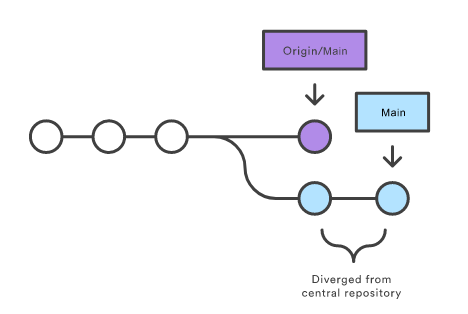
\includegraphics[width=.7\textwidth]{diverge}
\end{center}
In this situation, person B will need to rebase by pulling person A's commits into their local repository, integrate these changes locally, then pushing to the remote. One way to do this is as follows
\paragraph{git pull -- rebase origin main}
Which will pull all of the latest commits in main into your  
\subsection{Every Feature Gets a Branch}
A setup that is slightly more complicated to setup, but helps deal with issues that arise when multiple contributors are working on features at the samet ime and the inherent issue of needing to rebase the repository if someone else pushes their commits after you pull. 

\begin{center}
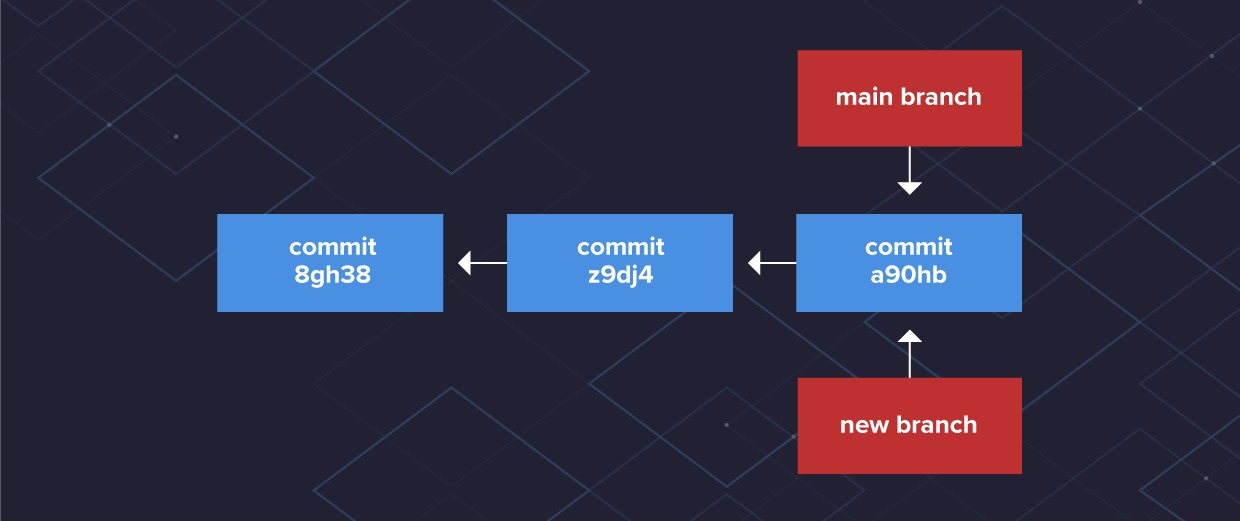
\includegraphics[width=\textwidth]{merge_picture.jpg}
\end{center}

\section{SyntaxCheat Sheet}
\subsection{git init [repository name]}
creates a new repository
\subsection{git add [file name]}
Stages changes. follow add with whatever changed/added files you want to stage, or just follow with a period to do everything (I only ever do this)
\subparagraph{git add .}

\subsection{git commit -m [commit message]}
commits the staged changes
\subsection{git pull}
makes a pull request
\subsection{git push}
pushes current commits to the remote repository
\subsection{git checkout [branch you want to switch to]}
Switches branches. If you specify a commit on the current branch you're currently on (and a branch doesn't already exist with that name) then it creates a new branch at that commit point with the name of that commit.
	\subparagraph{git checkout -b [branch name]}
	Creates a new branch called "branch name" that is a copy of the branch you're currently on.
\subsection{git merge}
merges branches together to, for example, merge a development branch to the main branch.
\end{document}